
\section{Experiments}
We next present the experimental results of \prorlagent across different tasks. We also perform in-depth investigations to provide a better understanding of our infrastructure.

\subsection{Experimental Setup}

Unless otherwise specified, we adopt DAPO~\citep{yu2025dapoopensourcellmreinforcement} as the default RL algorithm which filters out instances that are either too easy (resolved ratio 100\%) or too hard (resolved ratio 0\%).
We use a batch size of 32, a mini-batch size of 8, and generate 8 rollouts per instance. 
Rollouts with errors are excluded from gradient computation. The KL coefficient is set to $1\times10^{-4}$ and the learning rate to $1\times10^{-6}$. All RL training is performed on 32 NVIDIA H100 GPUs. 

\begin{table}[htb]
\centering
\small
\caption{Comparison of performance on SWE-Bench Verified across models of different scales. We report the reproduced performance and, where available, the reported results from prior work. Across all model sizes}
\label{tab:swe_results}
\setlength{\tabcolsep}{6pt}
\renewcommand{\arraystretch}{1.1}
\begin{tabular*}{\linewidth}{@{\extracolsep{\fill}}llcc@{}}
\toprule
\textbf{Size} & \textbf{Model} & \textbf{Reproduced} & \textbf{Reported} \\
\midrule
\multirow{2}{*}{4B} 
& Qwen3-4B-Instruct-2507        & 14.8 & --   \\
& \cellcolor{gray!30} \textbf{ProRL Agent-4B (RL)}  & \cellcolor{gray!30}\textbf{21.2} & \cellcolor{gray!30}--   \\
\midrule
\multirow{3}{*}{8B} 
& Qwen3-8B                      & 9.6  & --   \\
& SkyRL-Agent-8B-v0             & --   & 9.4  \\
& \cellcolor{gray!30}\textbf{ProRL Agent-8B (RL)}  & \cellcolor{gray!30}\textbf{18.0} & \cellcolor{gray!30} --   \\
\midrule
\multirow{3}{*}{14B} 
& Qwen3-14B                     & 15.4 & --   \\
& SkyRL-Agent-14B-v0            & --   & 21.6 \\
& \cellcolor{gray!30} \textbf{ProRL Agent-14B (RL)} & \cellcolor{gray!30} \textbf{23.6} & \cellcolor{gray!30} --   \\
\bottomrule
\end{tabular*}
\end{table}


\subsection{Main Results on Software Engineering}

We primarily evaluate \prorlagent on software engineering tasks. Specifically, we train Qwen3-4B-Instruct-2507, Qwen3-8B, and Qwen3-14B on the 293-instance subset of SWE-Gym used in SkyRL-v0~\citep{cao2025skyrl}. For the thinking models, Qwen3-8B and Qwen3-14B, we enable thinking mode during training. The results are reported in Table~\ref{tab:swe_results}.

As shown in Table~\ref{tab:swe_results}, \prorlagent consistently improves performance across all model sizes. Compared with SkyRL-v0~\citep{cao2025skyrl}, the gains are particularly notable for the 8B model, where \prorlagent achieves nearly a 2$\times$ improvement on SWE-Bench Verified. These results suggest that our infrastructure provides a more effective and stable foundation for RL training on software engineering agents.


\subsection{Generality Across Agent Domains}
Beyond software engineering agents, we further demonstrate the generality of \prorlagent by conduct RL training on other domains. \\
\noindent\textbf{STEM Agent.}
We further train a STEM agent designed to solve complex question-answering tasks across science, technology, engineering, and mathematics. Its primary tool is \emph{web search}, which enables retrieval of external knowledge for open-domain reasoning. In addition, the agent is equipped with the Bash and IPython tools provided by our infrastructure, allowing it to write and execute code for numerical computation and symbolic problem solving.
For the web search backend, we use Tavily. For training data, we follow the ProRL recipe~\citep{prorl2025} and use the SCP-116K dataset~\citep{lu2025scp116khighqualityproblemsolutiondataset}.

As shown in \Cref{fig:stem_agent}, the mean reward increases steadily throughout RL training, rising from approximately 0.2 to around 0.65 after 60 training steps. The smoothed curve maintains a clear upward trend without signs of saturation, suggesting that additional training may lead to further gains. These results demonstrate that \prorlagent extends naturally beyond software engineering tasks, requiring only appropriate tool configurations and reward designs for new domains.


\noindent\textbf{Math Agent.} 
We also train a math agent to solve mathematical problems. Following ProRL~\citep{prorl2025} we use DeepScaleR~\citep{deepscaler2025} data for training and further instruct models to use tools to solve and verify its own answers. Its primary tool is \emph{IPython execution}, which provides a full computational environment with preloaded libraries such as NumPy, SciPy, and SymPy for numerical analysis and symbolic manipulation. In addition, the agent is equipped with a \texttt{think} tool for explicit planning, enabling it to decompose complex problems, devise solution strategies, and iteratively verify answers through computation. The execution backend is implemented with an IPython kernel with pre-installed scientific libraries provided by our infrastructures.

As shown in \Cref{fig:math_agent}, the Pass@1 performance on AMC improves steadily during RL training, increasing from 0.4 to approximately 0.9. The relatively low initial performance reflects the fact that the base model is not yet proficient at solving mathematical problems through simple tool use. Through RL training with \prorlagent, agent learns to effectively leverage external tools for mathematical reasoning and achieves substantial performance gains

\begin{figure*}[t]
  \centering
  \begin{subfigure}[t]{0.32\textwidth}
    \centering
    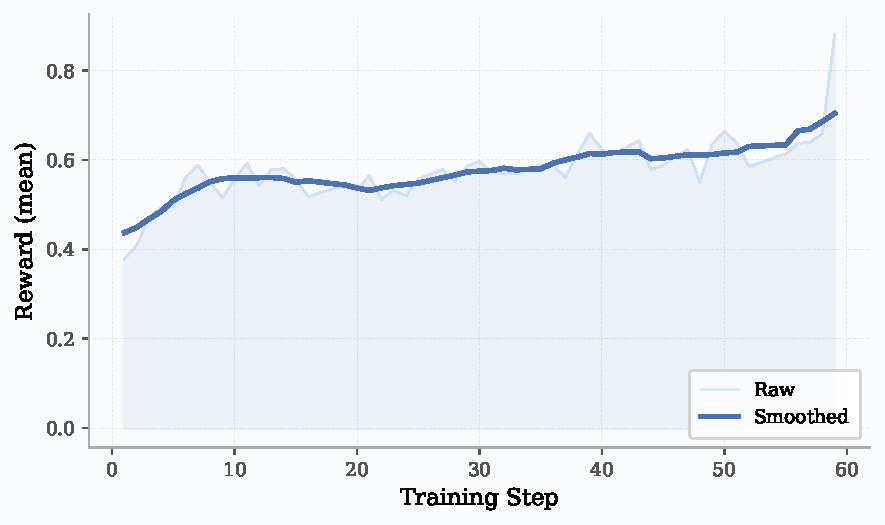
\includegraphics[width=\linewidth]{figures/stem_agent_reward.pdf}
    \caption{STEM agent.}
    \label{fig:stem_agent}
  \end{subfigure}
  \hfill
  \begin{subfigure}[t]{0.32\textwidth}
    \centering
    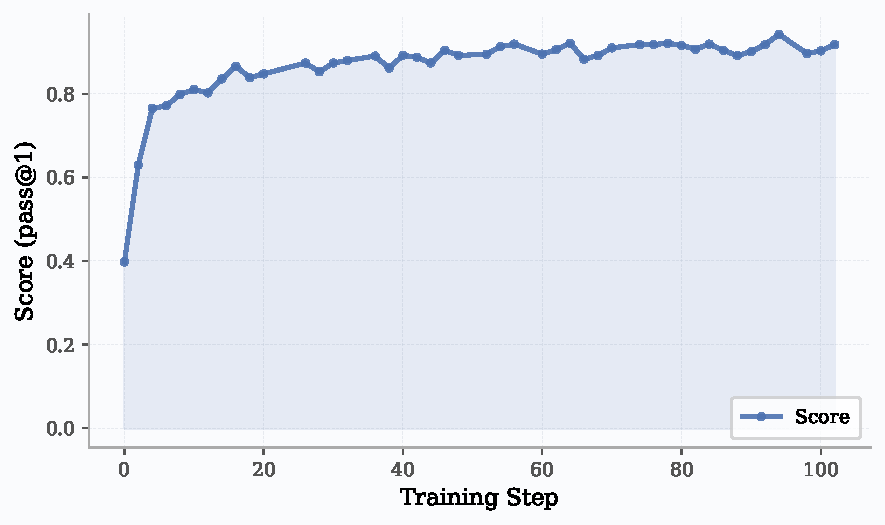
\includegraphics[width=\linewidth]{figures/math_training_curve.pdf}
    \caption{Math agent.}
    \label{fig:math_agent}
  \end{subfigure}
  \hfill
  \begin{subfigure}[t]{0.32\textwidth}
    \centering
    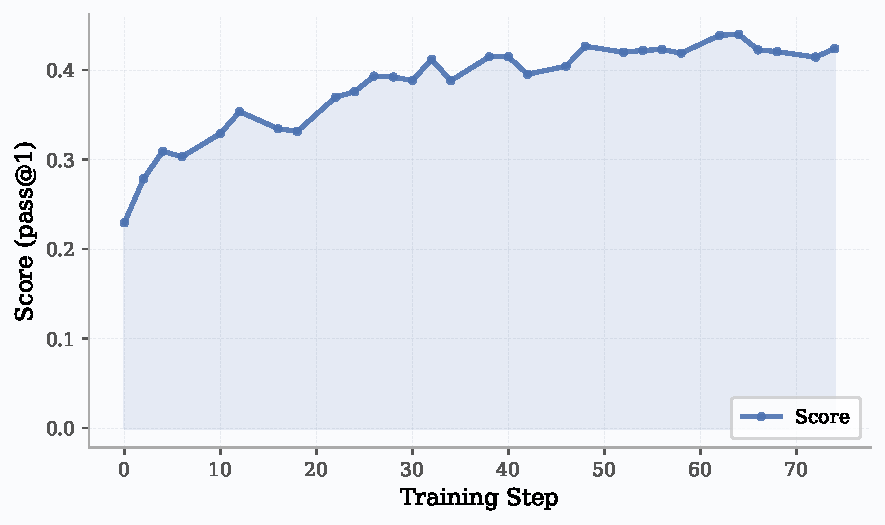
\includegraphics[width=\linewidth]{figures/code_score_curve.pdf}
    \caption{Code agent.}
    \label{fig:code_agent}
  \end{subfigure}
  \caption{Training curves for \prorlagent across three agent domains. From left to right: mean reward during RL training of the STEM agent, Pass@1 on AMC during RL training of the math agent, and Pass@1 on Codeforces during RL training of the code agent. All three curves show steady improvement during training, demonstrating the generality of \prorlagent beyond software engineering tasks.}
  \label{fig:other_agents}
\end{figure*}


\noindent\textbf{Code Agent.} 
We also train a code agent for program synthesis tasks. Following ProRL~\citep{prorl2025} we use Eurus-2-RL-Data~\citep{yuan2024implicitprm} as the training data and evaluate on the testing split of Codeforces. The primary tool is \emph{file editing via \texttt{str\_replace\_editor}}, which enables precise modification of source code in a dedicated \texttt{/workspace/solution.py} file. In addition, the agent is equipped with Bash execution for running test scripts and IPython tools for rapid prototyping, allowing it to iteratively develop, test, and debug solutions.
We adopt a test-driven training setup in which the agent writes verification scripts and validates outputs against expected results provided together with the problem statement. We explicitly instruct the model to verify candidate solutions with tests before submission. For reward computation, we extract the final solution from \texttt{/workspace/solution.py} and evaluate it using hidden test cases.


As shown in \Cref{fig:code_agent}, the Pass@1 performance on Codeforces improves steadily during RL training, increasing from 0.23 to approximately 0.42. Similar to the math agent, the base model initially struggles with effective use of the \texttt{str\_replace\_editor} tool and test-based verification. RL training substantially improves these capabilities, demonstrating that \prorlagent can effectively learn code generation through tool use.


\begin{table}[htb]
\centering
\small
\setlength{\tabcolsep}{5pt}
\renewcommand{\arraystretch}{1.08}
\caption{Ablation study of the proposed system components. Action Time denotes the average time required to execute shell-command actions. Each component improves rollout throughput, either by increasing GPU utilization or by reducing action execution time.}
\begin{tabular*}{\linewidth}{@{\extracolsep{\fill}}cccccc@{}}
\toprule
\textbf{Load Balancing} & \textbf{Efficient Bash}  & \textbf{Stale Job Cleanup} & \textbf{Action Time (s)} & \textbf{GPU Util (\%)} & \textbf{Throughput (instance/sec)} \\
\midrule 
\rowcolor{gray!30} \checkmark &  \checkmark   &  \checkmark  &      0.42       &          78 &    0.37        \\
     &  \checkmark   &  \checkmark  &       0.42      &   42        &       0.25     \\
          \checkmark &     &  \checkmark  &     0.78        &    68       &    0.29        \\
               \checkmark &  \checkmark   &   &        0.42     &          65 &    0.30        \\
     
   \bottomrule
\end{tabular*}
\label{tab: ablation}
\end{table}

\subsection{System Analysis}

\subsubsection{Scalability Across Compute Nodes}



To evaluate the scalability of \prorlagent, we measure rollout throughput (instances per second) on software engineering tasks as the number of compute nodes increases. The results are shown in Fig.~\ref{fig:throughput}.

As shown in Fig.~\ref{fig:throughput}, throughput increases nearly linearly with the number of nodes, indicating that \prorlagent can effectively leverage additional compute resources with minimal scaling overhead. This scalability is particularly valuable for RL training, where efficient rollout generation is often the main system bottleneck and directly affects overall training efficiency.
\begin{figure}[t]
  \centering
  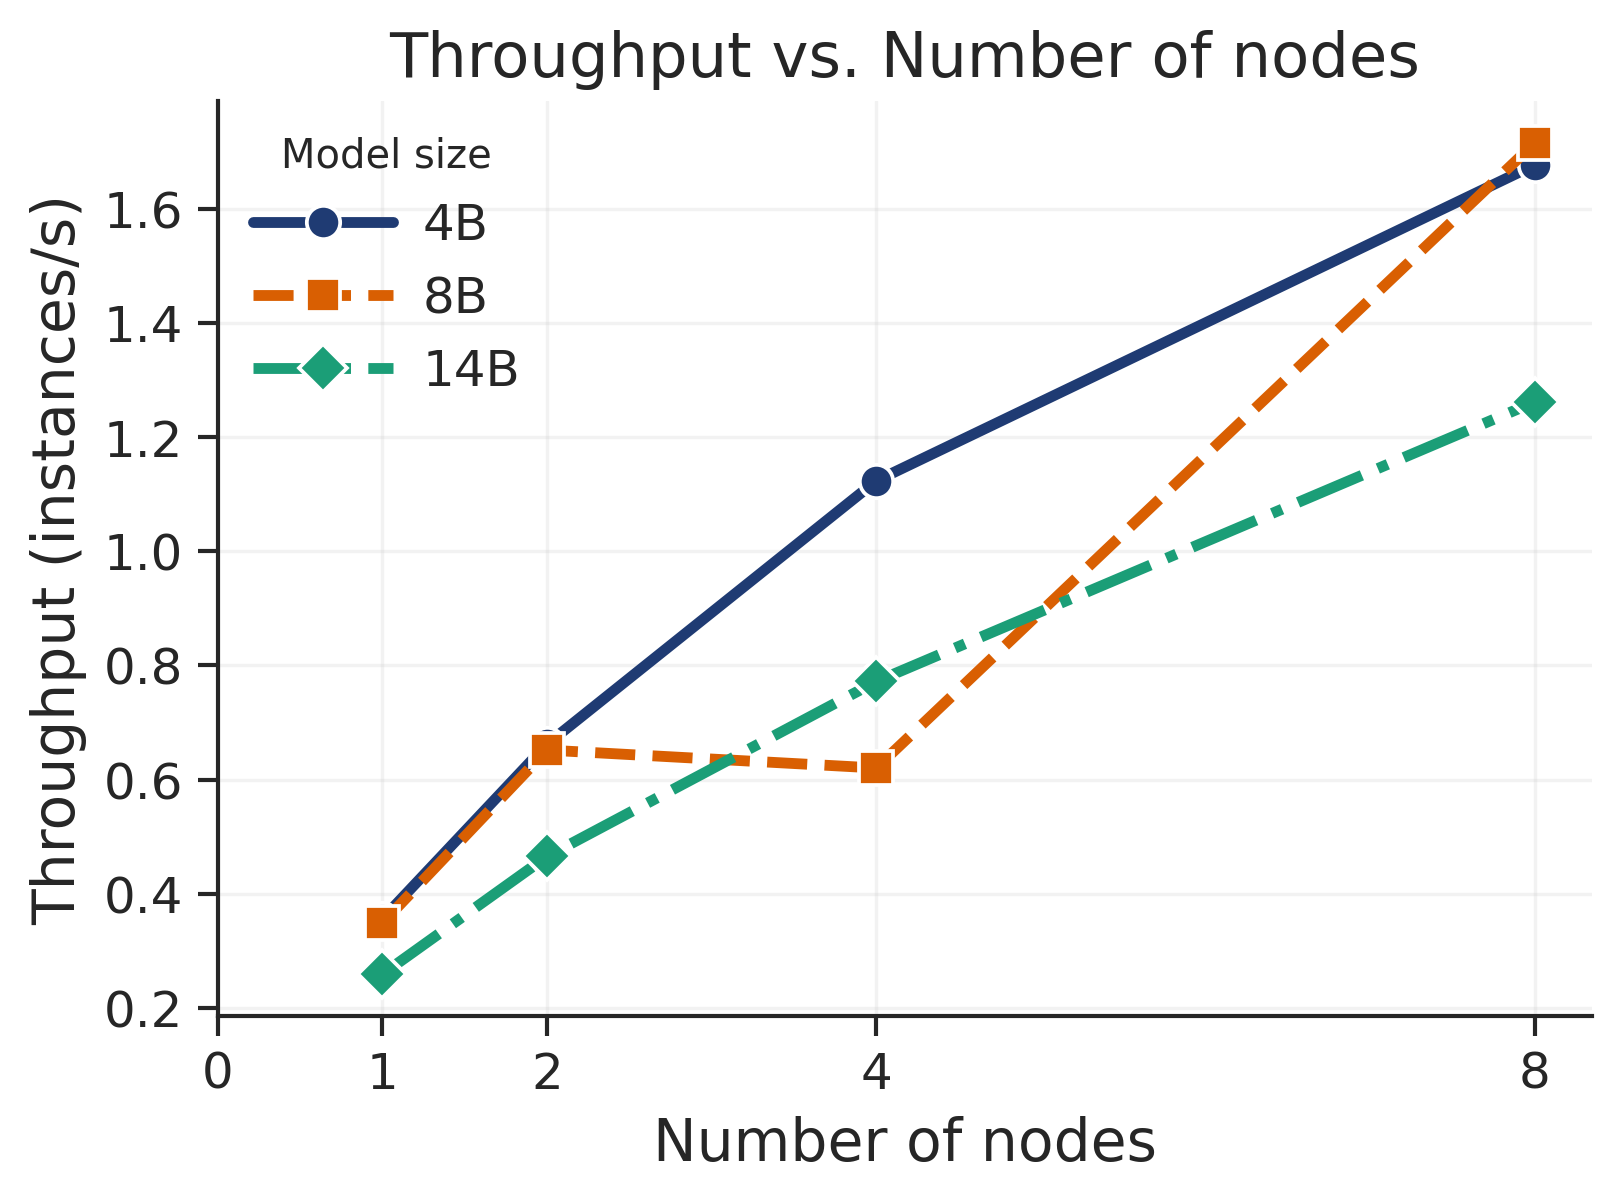
\includegraphics[width=0.55\textwidth]{figures/fig4_throughput.png}
\caption{Rollout throughput (instances/sec) on software engineering tasks versus the number of compute nodes. The near-linear increase in throughput demonstrates that \prorlagent scales efficiently with additional compute resources.}
  \label{fig:throughput}
\end{figure}
\subsubsection{Component Ablations}
We then conducted ablation experiments to evaluate the effectiveness of key components of the ProRL Agent including Load Balancing (LB), Efficient Bash (EB), Stale job Cleanup (SC). 
Specifically, we measure the rollout throughput of DAPO training on Qwen3-14B-Instruct-2507 using 8 H100 GPUs, with each component removed in turn. For the variant without Load Balancing, we use a simple baseline assignment strategy that distributes an equal 
number of instances to each LLM server. For the variant without Efficient Bash, we replace our optimized implementation with the original Bash implementation from OpenHands~\citep{wang2024openhands}. For the variant without Stale Job Cleanup, we wait for all jobs to finish before proceeding.
The results in \Cref{tab: ablation} show that each proposed component contributes to higher rollout throughput during DAPO training. In particular, Load Balancing and Stale Job Cleanup improve throughput by increasing GPU utilization, while Efficient Bash improves throughput by reducing action execution time.



